% !TeX program = xelatex
\documentclass[11pt]{article}
% =====================================================================
% Shared preamble for the Mal Customer 360 & CAR deliverable set.
% Compiled with: xelatex
% Palette is derived from the Mal logo (violet -> blue gradient), with
% darker, readable shades used for any text/UI role -- the bright
% gradient tones stay reserved for the logo image itself.
% =====================================================================

\usepackage{geometry}
\geometry{a4paper, top=2.4cm, bottom=2.6cm, left=2.3cm, right=2.3cm, headheight=26pt, headsep=12pt, footskip=32pt}

\usepackage{fontspec}
\usepackage{polyglossia}
\setmainlanguage{english}
% polyglossia (fontspec's standard hyphenation companion under XeLaTeX)
% activates real English hyphenation patterns -- without it, long words in
% narrow table columns have no valid break point and can overrun the
% column width instead of wrapping.
% Fonts are loaded from a project-local folder by file path, not by OS font-
% name lookup -- this makes the document compile identically on any machine
% (no system-wide font install, no admin rights, no "font not found" from
% fontspec querying a font book that doesn't have these registered) as long
% as fonts/ sits next to this preamble file. Path is resolved relative to
% the directory xelatex is invoked from, which for every document in this
% set is one level below this preamble (doc1_architecture/, doc2_erd/,
% doc3_sql/) -- hence "../fonts/" throughout.
\defaultfontfeatures{Path = ../fonts/, Extension = .ttf}
\setmainfont{LiberationSerif}[
  UprightFont = *-Regular, BoldFont = *-Bold,
  ItalicFont = *-Italic, BoldItalicFont = *-BoldItalic,
  Mapping=tex-text
]
\newfontfamily\headfont{LiberationSans}[
  UprightFont = *-Regular, BoldFont = *-Bold,
  ItalicFont = *-Italic, BoldItalicFont = *-BoldItalic, Mapping=tex-text
]
\newfontfamily\uifont{LiberationSans}[
  UprightFont = *-Regular, BoldFont = *-Bold,
  ItalicFont = *-Italic, BoldItalicFont = *-BoldItalic, Mapping=tex-text
]
\setmonofont{DejaVuSansMono}[
  UprightFont = *, BoldFont = *-Bold,
  ItalicFont = *-Oblique, BoldItalicFont = *-BoldOblique,
  Scale=0.86
]

% A \texttt{snake_case_identifier} is otherwise one unbreakable "word" to
% TeX -- long column/table names in \texttt{} routinely overran a table
% cell or the right margin with no valid break point. Letting a line
% break after each underscore fixes that at the source (every overfull
% hbox in this document set traced back to exactly this) without
% changing how the identifier renders when a break isn't needed.
\let\malorigunderscore\_
\renewcommand{\_}{\malorigunderscore\allowbreak}

% Absorbs the small (sub-20pt) overfull/underfull hboxes that show up in
% justified body text and code comments via micro-scale font expansion --
% cheaper and less fragile than hand-patching individual line breaks.
\usepackage{microtype}

\usepackage[table]{xcolor}

% ---------- Brand palette (sampled from the logo: violet #AC54DF -> blue #44B9EF) ----------
\definecolor{malprimary}{HTML}{5B2C8F}       % deep violet -- headings, links, primary accents
\definecolor{malprimarystrong}{HTML}{3B1B63} % darker violet -- small text needing extra contrast
\definecolor{malaccent}{HTML}{1868A3}        % deep blue (logo's blue side) -- secondary accent
\definecolor{malink}{HTML}{201A33}           % near-black, slight violet cast -- primary body text
\definecolor{malmuted}{HTML}{473F5C}         % dark violet-grey -- secondary text (still high contrast)
\definecolor{malfaint}{HTML}{6E6480}         % medium violet-grey -- incidental text only (footers, page numbers), NEVER body content
\definecolor{malline}{HTML}{DED3EC}          % light lavender -- decorative hairlines
\definecolor{maltableline}{HTML}{B7A6CE}     % visible medium lavender-grey -- table borders
\definecolor{malwash}{HTML}{F2EDFA}          % very light lavender wash -- callout backgrounds
\definecolor{malwashdeep}{HTML}{E4D6F5}      % deeper lavender wash -- box accents
\definecolor{malheaderwash}{HTML}{ECE1F8}    % table header-row shading

% ---------- Code block colors ----------
\definecolor{malcodebg}{HTML}{1B1330}
\definecolor{malcodetext}{HTML}{EDE7F7}
\definecolor{malcodecomment}{HTML}{8B93C9}
\definecolor{malcodekeyword}{HTML}{86C6F2}

% ---------- Semantic tier badge colors (meaning, not brand -- left as a
% traffic-light-style progression of sensitivity) ----------
\definecolor{malsafebg}{HTML}{DCEFE6}
\definecolor{malsafetext}{HTML}{1B5E4F}
\definecolor{malamberbg}{HTML}{F5E7C7}
\definecolor{malambertext}{HTML}{8A6414}
\definecolor{malcritbg}{HTML}{F6DCC9}
\definecolor{malcrittext}{HTML}{8F4A1F}

\usepackage{parskip}
\setlength{\parskip}{7pt}
\setlength{\parindent}{0pt}

\usepackage{titlesec}
% Section numbers render as a small filled "chip" -- a deliberate nod to a
% presentation-deck agenda item rather than a plain research-paper numeral.
\titleformat{\section}
  {\headfont\Large\bfseries\color{malink}}
  {\colorbox{malprimary}{\raisebox{0.1ex}{\makebox[1.7em][c]{\color{white}\thesection}}}}
  {0.7em}{}
\titlespacing*{\section}{0pt}{1.8em}{0.9em}
\titleformat{\subsection}
  {\headfont\large\bfseries\color{malink}}
  {\color{malprimary}\thesubsection}{0.6em}{}
\titlespacing*{\subsection}{0pt}{1.4em}{0.55em}
\titleformat{\subsubsection}
  {\headfont\normalsize\bfseries\color{malprimarystrong}}
  {}{0em}{}
\titlespacing*{\subsubsection}{0pt}{1.2em}{0.4em}

\usepackage{enumitem}
\setlist{topsep=3pt, itemsep=4pt, parsep=0pt, leftmargin=1.3em}

\usepackage{booktabs}
\usepackage{array}
\usepackage{longtable}
\usepackage{caption}
\captionsetup{font={sf,small,color=malmuted}, labelfont={bf,color=malprimarystrong}, margin=0pt}

% More generous row height everywhere a table appears -- addresses cramped
% header/value spacing. Combined with \arrayrulecolor, every table below
% also gets a full visible grid rather than relying on booktabs alone.
\renewcommand{\arraystretch}{1.35}
\arrayrulecolor{maltableline}

% Author / contact line shown in the footer of every page. Edit this one
% line to change the name and email across all three documents at once.
\newcommand{\DocAuthorLine}{Adithya Menon \textbullet\ amenon3002@gmail.com}

\usepackage{fancyhdr}
\pagestyle{fancy}
\fancyhf{}
\renewcommand{\headrulewidth}{0.5pt}
\renewcommand{\footrulewidth}{0pt}
\fancyhead[L]{\uifont\footnotesize\color{malmuted}\DocKicker}
\fancyhead[R]{\raisebox{-0.2cm}{
\includegraphics[height=0.55cm]{../assets/mal-logo}}}
\fancyfoot[L]{\uifont\footnotesize\color{malfaint}\DocFooterTag}
\fancyfoot[C]{\uifont\footnotesize\color{malfaint}\DocAuthorLine}
\fancyfoot[R]{\uifont\footnotesize\color{malfaint}\thepage}
\renewcommand{\headrule}{{\color{malline}\hrule height\headrulewidth}}

\usepackage{tcolorbox}
\tcbuselibrary{skins,breakable}

% "Why this way" -- the introspective / design-rationale callout used
% throughout every deliverable to explain reasoning, not just state facts.
% NOTE: "attach title to upper" needs an explicit separator (a colon plus
% a real space) below -- without one, the title text runs directly into
% the body text with no gap at all.
\newtcolorbox{rationale}[1][]{%
  breakable, enhanced, colback=malwash, colframe=malline,
  boxrule=0.4pt, left=10pt, right=10pt, top=7pt, bottom=7pt,
  borderline west={2.6pt}{0pt}{malprimary},
  fonttitle=\headfont\bfseries\footnotesize,
  coltitle=malprimarystrong,
  before upper={\uifont\small},
  title={\MakeUppercase{Why This Way}#1},
  attach title to upper={:\ \ },
  title after break=\MakeUppercase{Why This Way (cont.)},
}

% Pseudo data-example box (looks like a small terminal / record card)
\newtcolorbox{datarecord}[1]{%
  breakable, enhanced, colback=malcodebg, colframe=malcodebg,
  boxrule=0pt, arc=3pt, left=11pt, right=11pt, top=8pt, bottom=8pt,
  fonttitle=\uifont\bfseries\footnotesize, coltitle=malcodetext,
  colbacktitle=malprimarystrong,
  title={#1},
}

% Flat fact / caveat box
\newtcolorbox{note}[1][Note]{%
  breakable, enhanced, colback=white, colframe=malaccent,
  boxrule=0.6pt, arc=2pt, left=9pt, right=9pt, top=6pt, bottom=6pt,
  fonttitle=\headfont\bfseries\footnotesize, coltitle=white, colbacktitle=malaccent,
  title={#1},
}

% Stakeholder-question box -- used throughout the trade-offs/Q&A
% deliverable. #1 = who is asking, #2 = the question itself (rendered
% italicized, in quotes, before the answer). Title bar is solid (unlike
% the plain colored-text title on `rationale') so a reader skimming the
% document can tell "why this way" asides apart from an actual posed
% question at a glance.
\newtcolorbox{stakeholderq}[2]{%
  breakable, enhanced, colback=malwash, colframe=malprimary,
  boxrule=0.6pt, arc=2pt, left=10pt, right=10pt, top=8pt, bottom=8pt,
  fonttitle=\headfont\bfseries\footnotesize, coltitle=white, colbacktitle=malprimary,
  title={\MakeUppercase{#1} ASKS},
  before upper={\uifont\small\itshape\color{malprimarystrong}``#2''\par\vspace{5pt}\upshape\normalfont\rmfamily\color{malink}},
}

% Plain, unattributed "Reference:" line -- used in the exam/test-paper-style
% Q&A document, where a question is answered directly rather than framed as
% asked by a named stakeholder.
\newcommand{\QARef}[1]{\par\smallskip\noindent{\footnotesize\color{malfaint}\textbf{Reference:} #1}}

\usepackage{listings}
\lstdefinelanguage{PseudoSQL}{
  morekeywords={SELECT,FROM,WHERE,JOIN,LEFT,RIGHT,INNER,OUTER,ON,AND,OR,AS,
    GROUP,BY,ORDER,HAVING,INSERT,INTO,VALUES,CREATE,TABLE,VIEW,MERGE,USING,
    WHEN,MATCHED,NOT,THEN,UPDATE,SET,DELETE,DISTINCT,UNION,ALL,WITH,CASE,
    ELSE,END,NULL,IS,IN,COALESCE,GREATEST,LEAST,VARCHAR,DECIMAL,TIMESTAMP,
    DATE,BOOLEAN,INT,FLOAT,PRIMARY,KEY,FOREIGN,REFERENCES,NOT,DEFAULT,
    PARTITION,FILTER,OVER,ROW_NUMBER,MODE,WITHIN,ATTACH,MASKING,POLICY,
    PRIORITY,TO,ROLE,CURRENT_ROLE,CURRENT_DATE,CURRENT_TIMESTAMP,INTERVAL,
    NULLIF,SUM,AVG,COUNT},
  sensitive=false,
  morecomment=[l]{--},
  morestring=[b]',
}
\lstdefinestyle{codeblock}{
  backgroundcolor=\color{malcodebg},
  basicstyle=\ttfamily\footnotesize\color{malcodetext},
  keywordstyle=\color{malcodekeyword}\bfseries,
  commentstyle=\color{malcodecomment}\itshape,
  stringstyle=\color{malcodetext},
  numbers=left, numberstyle=\tiny\color{malcodecomment}, numbersep=9pt,
  breaklines=true, breakatwhitespace=false,
  showstringspaces=false,
  frame=single, framerule=0pt, rulecolor=\color{malcodebg},
  framesep=8pt, xleftmargin=1.4em, xrightmargin=0.4em,
  aboveskip=9pt, belowskip=11pt,
  tabsize=2,
  columns=fullflexible,
}
\lstset{style=codeblock}

\usepackage{hyperref}
\hypersetup{
  colorlinks=true, linkcolor=malprimarystrong, urlcolor=malprimarystrong,
  citecolor=malprimarystrong,
  pdfstartview=FitH,
}

\usepackage{graphicx}
\usepackage{tabularx}
\newcolumntype{Y}{>{\raggedright\arraybackslash}X}
% Bordered, readable table columns -- used in place of bare Y/p{} columns
% wherever a table was flagged as hard to scan. L/C take an explicit width.
\newcolumntype{L}[1]{>{\raggedright\arraybackslash}p{#1}}
\newcolumntype{C}[1]{>{\centering\arraybackslash}p{#1}}

% Shades the header row of a bordered table. \tblheadrow triggers the row
% background (safe -- \rowcolor is self-scoped and never leaks); each
% header cell is then wrapped individually with \hcell{...}, which opens
% its own brace group so the white/bold styling can never leak sideways
% into the next cell or downward into the data rows below it -- the same
% class of color-scope bug documented in the title-page macro above.
% Usage: \tblheadrow \hcell{Pass} & \hcell{Key} & \hcell{Basis} & \hcell{Confidence} \\ \hline
\newcommand{\tblheadrow}{\rowcolor{malprimary}}
\newcommand{\hcell}[1]{{\color{white}\bfseries #1}}

% ---------- Tag-style badges for tiers, used inside tables ----------
\newcommand{\tierzero}{\colorbox{malsafebg}{\textcolor{malsafetext}{\scriptsize\bfseries\ Tier 0\ }}}
\newcommand{\tierone}{\colorbox{malamberbg}{\textcolor{malambertext}{\scriptsize\bfseries\ Tier 1\ }}}
\newcommand{\tiertwo}{\colorbox{malcritbg}{\textcolor{malcrittext}{\scriptsize\bfseries\ Tier 2\ }}}
\newcommand{\tierthree}{\colorbox{malcrittext!85}{\textcolor{white}{\scriptsize\bfseries\ Tier 3\ }}}

% ---------- Title block ----------
\newcommand{\DocKicker}{}
\newcommand{\DocFooterTag}{}
\newcommand{\malTitlePage}[5]{%
  % #1 kicker, #2 title, #3 subtitle/dek, #4 part-of-N label, #5 meta rows (tabularx content)
  \renewcommand{\DocKicker}{#1}
  \thispagestyle{empty}
  \begingroup
  \raggedright
  \vspace*{-1.0cm}
  \noindent
  \begin{minipage}[t]{0.75\linewidth}
    \raggedright
    {\uifont\small\color{malaccent}\bfseries\MakeUppercase{#1}}\\[10pt]
    {\headfont\huge\bfseries\color{malink} #2}\\[10pt]
    {\uifont\color{malmuted}\large #3}
  \end{minipage}%
  \hfill
  \begin{minipage}[t]{0.17\linewidth}
    \raggedleft
    
\includegraphics[width=\linewidth]{../assets/mal-logo}
  \end{minipage}
  \\[16pt]
  {\uifont\footnotesize\color{malprimarystrong}\bfseries #4}\\[14pt]
  {\color{malline}\hrule height 0.6pt}
  \vspace{12pt}
  % Explicit dark color + extra row spacing on the meta block itself, so a
  % missing per-document \color never again silently inherits a leftover
  % (pale, hairline-only) color from whatever ran immediately before it.
  {\uifont\small\color{malink}\renewcommand{\arraystretch}{1.6}#5}
  \vspace{8pt}
  {\color{malline}\hrule height 0.6pt}
  \vspace{18pt}
  \endgroup
}


\begin{document}
\renewcommand{\DocFooterTag}{Deliverable 2 of 3}

\malTitlePage
  {Mal \textbullet\ Data Platform \textbullet\ Deliverable 2 of 3}
  {Customer 360 \& CAR: Entity-Relationship Diagram}
  {The complete field-level schema for the golden Customer 360 and the CAR snapshot, drawn as one connected model, with an entity dictionary and a cardinality walkthrough for engineers who need to build against it directly.}
  {DELIVERABLE 2 OF 3 --- ERD}
  {\begin{tabular}{|L{3.6cm}|L{4.6cm}|L{2.3cm}|L{3.7cm}|}
    \hline
    \tblheadrow \hcell{Companion Documents} & \hcell{Notation} & \hcell{Status} & \hcell{Targets} \\
    \hline
    \#1 Architecture \quad \#3 Identity SQL & Crow's foot (Mermaid \texttt{erDiagram}) & Draft for review & 500K customers, Year 1 \\
    \hline
  \end{tabular}}

\section*{How to Read This Diagram}
\addcontentsline{toc}{section}{How to Read This Diagram}
This diagram uses standard crow's-foot notation. A single bar means \emph{exactly one}; a circle means \emph{zero, optionally}; a crow's foot (three prongs) means \emph{many}. Reading the notation at the end nearest an entity tells you the cardinality \emph{from the other entity's point of view} -- so \texttt{CUSTOMER\_GOLDEN\ ||--o\{\ ACCOUNT} reads as "one customer owns zero or many accounts."

Solid connecting lines are enforced foreign keys inside the golden layer. \texttt{CAR\_SNAPSHOT} is drawn as a satellite of Customer rather than a peer of the other entities because it is a derived, denormalized artifact rebuilt nightly from everything else in this diagram -- nothing else holds a live foreign key into it, and it holds none into anything but Customer.

\begin{figure}[h]
\centering
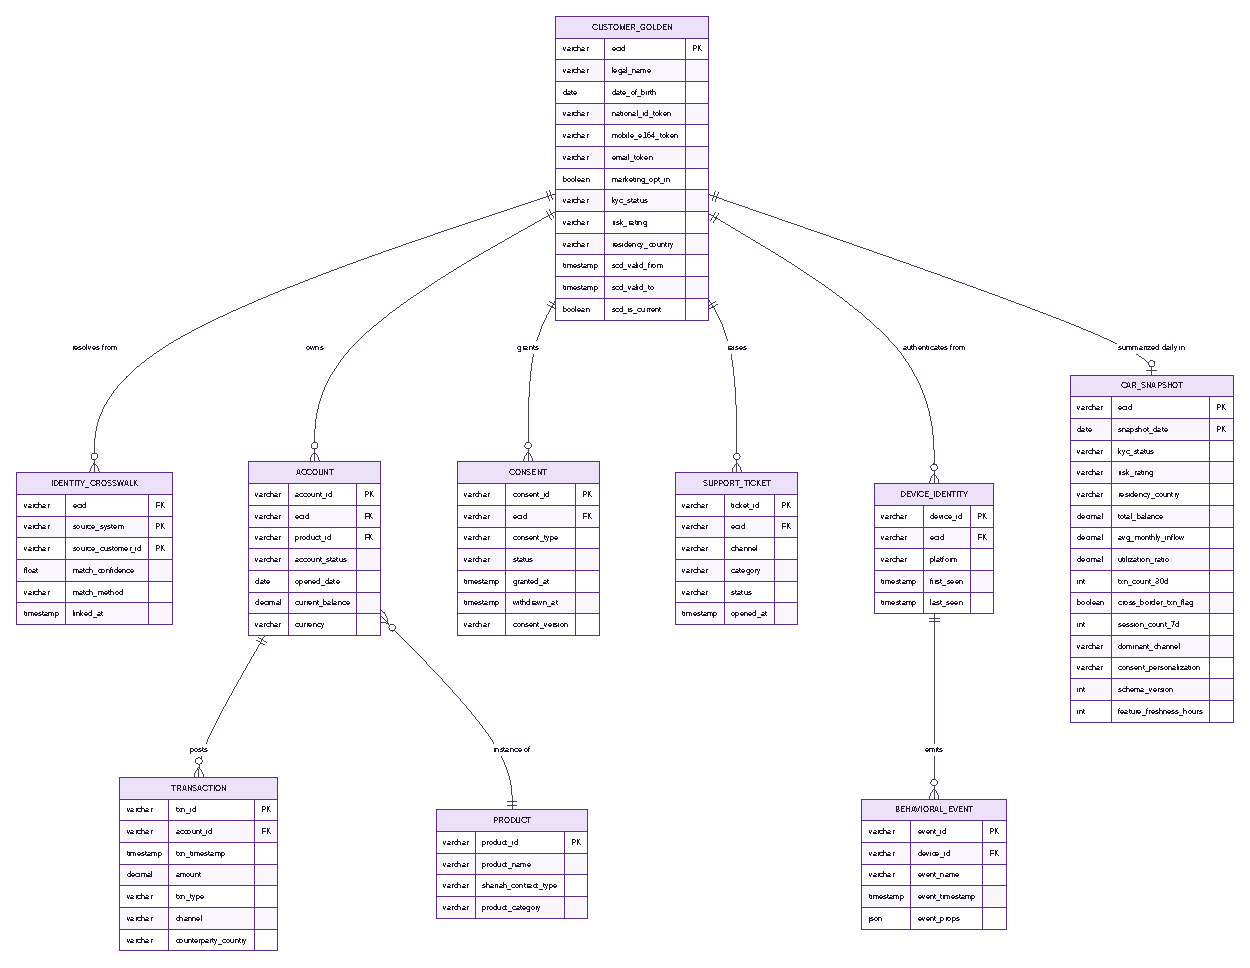
\includegraphics[width=\linewidth]{erd.pdf}
\caption{Golden Customer 360 core plus the CAR snapshot. Rendered from Mermaid \texttt{erDiagram} source; entity and column names match the SQL in Deliverable 3 exactly.}
\end{figure}

\clearpage
\section{Entity Dictionary}
Each entity below is described by what one row actually represents (its grain), its role in the schema (dimension, fact, bridge, or derived), and the fields worth calling out specifically.

\subsection{CUSTOMER\_GOLDEN --- The Golden Identity Dimension}
\textbf{Grain:} one row per Enterprise Customer ID (ECID) per version. \textbf{Role:} SCD Type 2 dimension -- the single source of truth for who a customer is. \texttt{ecid} is generated once, at first resolution, and never changes; \texttt{scd\_valid\_from} / \texttt{scd\_valid\_to} / \texttt{scd\_is\_current} track history so that "what did we know about this customer on this date" is always answerable, which matters for audit and for avoiding label leakage in model training. \texttt{national\_id\_token}, \texttt{mobile\_e164\_token}, and \texttt{email\_token} are tokenized, never raw, values -- see Deliverable 1, Section 4. \texttt{marketing\_opt\_in} is the one field on this table that core banking has no equivalent for and never overwrites -- per the survivorship rules in Deliverable 1, Section 2.3, it always survives from CRM.

\subsection{IDENTITY\_CROSSWALK --- The Merge Ledger}
\textbf{Grain:} one row per (source system, source customer ID) pair. \textbf{Role:} bridge table, and the actual mechanism behind every merge and split. This table, not \texttt{CUSTOMER\_GOLDEN}, is what identity resolution writes to -- an ECID's membership is defined by which crosswalk rows point to it, which is what makes an incorrect merge reversible: correcting it is a crosswalk update and an SCD2 replay, not a destructive rewrite of the golden record itself.

\subsection{ACCOUNT --- The Banking Relationship}
\textbf{Grain:} one row per account (current, savings, financing). \textbf{Role:} dimension, owned by exactly one \texttt{ecid} for Q2 (joint accounts are a Year 2 extension, modeled as an additional bridge rather than a change to this table). References \texttt{PRODUCT} rather than repeating product attributes on every account row.

\subsection{PRODUCT --- The Catalog}
\textbf{Grain:} one row per product definition. \textbf{Role:} dimension. Carries \texttt{shariah\_contract\_type} (Murabaha, Mudarabah, Wakala, and so on) instead of an interest rate -- the one place this schema visibly departs from a conventional-bank Customer 360 template, because the underlying contract structure is what both Product and Compliance actually need to reason about.

\subsection{TRANSACTION --- The Posted Ledger}
\textbf{Grain:} one row per posted transaction. \textbf{Role:} fact table, additive, referencing \texttt{ACCOUNT}. Kept at transaction grain in the 360 for Support and Product to answer "what happened"; heavier aggregation for scoring happens downstream in \texttt{CAR\_SNAPSHOT}, not here.

\subsection{CONSENT --- The Single Gate}
\textbf{Grain:} one row per (\texttt{ecid}, consent type, version). \textbf{Role:} dimension-like control table. Every masking and personalization decision in the platform reads from this table; nothing downstream is allowed to maintain its own separate notion of whether a customer has agreed to something.

\subsection{SUPPORT\_TICKET --- CRM Case History}
\textbf{Grain:} one row per case. \textbf{Role:} fact table, linked to \texttt{ecid} once the originating CRM contact resolves through the crosswalk.

\subsection{DEVICE\_IDENTITY --- The Authenticated Link to a Device}
\textbf{Grain:} one row per Amplitude device ID. \textbf{Role:} dimension, linked to \texttt{ecid} \emph{only} once an authenticated session confirms the device belongs to that customer -- never speculatively, never by behavioral inference alone.

\subsection{BEHAVIORAL\_EVENT --- Raw Amplitude Events}
\textbf{Grain:} one row per event. \textbf{Role:} fact table, referencing \texttt{DEVICE\_IDENTITY} rather than \texttt{ecid} directly, which is what makes the authenticated-binding rule in \texttt{DEVICE\_IDENTITY} the single enforcement point for the whole behavioral stream.

\subsection{CAR\_SNAPSHOT --- The Derived Analytic Record}
\textbf{Grain:} one row per (\texttt{ecid}, \texttt{snapshot\_date}). \textbf{Role:} derived, deliberately denormalized -- rebuilt nightly from every other entity in this diagram, never updated in place. It is intentionally the widest, flattest entity in the model; see Deliverable 1, Section 5 for why that width is the point rather than an oversight. \texttt{risk\_rating} and \texttt{residency\_country} are carried over unchanged from \texttt{CUSTOMER\_GOLDEN} rather than recomputed, and \texttt{feature\_freshness\_hours} records how stale the snapshot's inputs were at build time -- both exist so a model consuming this row never has to guess.

\section{Cardinality Walkthrough}
\begin{itemize}
\item \textbf{Customer \(\rightarrow\) Identity crosswalk (one to many):} one ECID can have many source-system linkages, one per system it appears in. This is the relationship merges and splits actually operate on.
\item \textbf{Customer \(\rightarrow\) CAR snapshot (one to at most one, per day):} zero or one row per ECID per \texttt{snapshot\_date} -- drawn as one-to-one because the "many" dimension here is time, not a second live relationship.
\item \textbf{Account \(\rightarrow\) Product (many to one):} many accounts can be instances of the same product; the Sharia contract type lives once, on \texttt{PRODUCT}, never repeated per account.
\item \textbf{Device identity \(\rightarrow\) Behavioral event (one to many):} raw Amplitude events, aggregated nightly into the CAR's engagement columns today, and consumed directly by the streaming layer once that exists.
\end{itemize}

\begin{rationale}
Every foreign key in this diagram points toward \texttt{ecid}, directly or through one hop, and never the reverse. That is a deliberate constraint, not a coincidence of how the boxes happened to get drawn: it keeps identity resolution upstream of everything else in the platform, so a change to how two records get matched only ever has to propagate forward through this diagram, never backward.
\end{rationale}

\end{document}
